\documentclass[letterpaper,spanish]{article}
\usepackage{babel}
\usepackage[latin1]{inputenc}
\usepackage[pdftex]{graphicx}
\usepackage[dvipsnames,usenames]{color}
\usepackage{fancyhdr}
\usepackage{latexsym}
\usepackage{verbatim}

\oddsidemargin -0.3cm \topmargin -1.1cm \headheight 2.5cm
\textwidth 16.8cm \textheight 19.8cm

\newsavebox{\fondo}
\sbox{\fondo}{
\includegraphics[keepaspectratio,height=1.35\textheight,width=1.35\textwidth]{../../02_publicimage/margin.png}}

\pagestyle{fancy}
\fancyhead[C]{\setlength{\unitlength}{1in}
\begin{picture}(0,0)\put(-3.9,-9.3){\usebox{\fondo}}\end{picture}}

\renewcommand{\headrulewidth}{0pt}
\title{\huge{\textbf{DOCUMENTO DE AN�LISIS \\ Componentes de gesti�n de espacios virtuales y materias}}}
\author{Yeah! S.R.L.}
\date{\small{9 de abril 2009}}

\begin{document}
\maketitle \pagebreak \tableofcontents \pagebreak

\section{INTRODUCCI�N}

Un recurso muy importante en un sistema de cursos y notas, son los espacios virtuales para las materias.

Por lo general, las materias se agrupan por areas, por ejemplo, las materias de Introducci\'on 
a la programaci\'on y Elementos de programaci\'on estan dentro del area de `Programaci\'on' mientras que las 
materias de Sistemas de Informaci\'on I y II estar\'an dentro del area de `Ingenier\'ia de Software'.

\section{DESCRIPCI\'ON DEL PROBLEMA}

Son conciderados espacios virtuales las:
\begin{itemize}
    \item Areas
    \item Materias
    \item Grupos
    \item Equipos
\end{itemize}

Cada una es mas general que otra y encierra a las de nivel inferior, cada uno de estos espacios virtuales 
tiene sus propios recursos como ser foros, anuncios, etc.

\section{DESCRIPCI�N DE LA SOLUCI\'ON}

El espacio virtual para las {\bfseries areas} se crear\'a de forma autom\'atica, es decir, cuando se crea 
una nueva materia se marca las areas a las que pertenece y se a\~nade a sus respectivos espacios, solo se crea 
un nuevo espacio cuando la materia que se crea no se relaciona con ninguna de las areas ya existentes.

\begin{figure}[h]
    \centering
        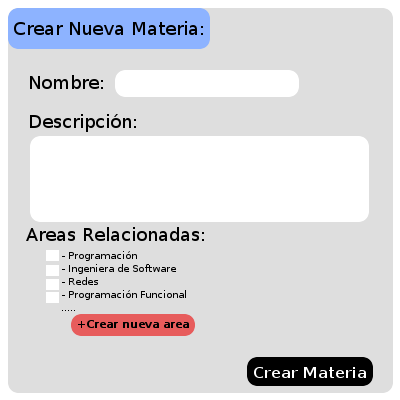
\includegraphics[width=0.4\textwidth]{images/crearMateria.png}
    \caption{Creaci\'on de una nueva materia}
    \label{fig:categorias}
\end{figure}

\section{MODULOS PROPUESTOS}

\begin{description}
    \item [SPACE] Controla y regula la creaci\'on autom\'atica de los espacios, evitando as\'i la 
    creacion descontrolada de este, ademas, se encarga de agrupar a las materias por sus areas relacionadas.
    \item [SUBJECT] Se encarga de manejar las materias la informaci\'on de estas y ademas se encarga de editar, crear y eliminar grupos.
    \item [GROUP] Controla la creaci\'on, modificaci\'on, y la informaci\'on referida a los grupos, ademas de la asignaci\'on de usuarios.
    \item [TEAM] Controla la creaci\'on, modificaci\'on, y la informaci\'on referida a los equipos de estudiantes(subgrupos) de cada grupo.

\end{description}

\section{FUNCIONES PROPUESTAS}
\subsection{SPACE}
    \begin {description}
        \item [Ver espacios] Lista todos los espacios con sus descripciones.
        \item [Editar espacios] Permite editar el t\'itulo y la descripci\'on del espacio.
    \end {description}
\subsection{SUBJECT}
    \begin {description}
        \item [Crear materia] Permite crear una nueva materia.
        \item [Ver materias] Lista todas las materias con un resumen de sus grupos y la descripci\'on de la 
        materia.
        \item [Editar materia] Permite editar el t\'itulo y la descripcion de la materia, y ademas de poder 
        eliminar a los grupos de la misma.
        \item [Cambiar estado a la materia] Las materias pueden tener un estado de habilitado o deshabilitado 
        como suele suceder en algunas materias electivas.
    \end {description}
\subsection{GROUP}
    \begin{description}
        \item [Crear grupos dentro de las materias] Permite creaci\'on de grupos.
        \item [Ver grupos] Lista todos los grupos con un resumen de los equipos que pertenecen a una materia 
        en especifico y la descripci\'on de la materia.
        \item [Editar grupo] Permite editar el t\'itulo, la descripci\'on del grupo, y ademas de poder 
        eliminar a los equipos de la misma.
        \item [Cambiar estado al grupo] Habilitado o Deshabilitado.

    \end{description}
\subsection{TEAM}
    \begin{description}
        \item [Crear equipos dentro de un grupo]
        \item [Ver equipos] Lista todos los equipos con sus integrantes.
        \item [Editar equipo] Permite editar el t\'itulo y la descripci\'on del equipo, y ademas de poder eliminar a los equipos de la misma.
        \item [Cambiar estado al equipo]

    \end{description}
\section{RESTRICCIONES ENCONTRADAS}
Ninguna.

\begin{comment}
\vspace{4cm}
    \begin{table}[htbp]
        \begin{center}
            \begin{tabular}{c c}
\_\_\_\_\_\_\_\_\_\_\_\_\_\_\_\_\_\_\_\_\_\_\_\_\_\_\_\_\_\_\_\_\_\_\_\_\_\_\_\_\_\_\_ &
\_\_\_\_\_\_\_\_\_\_\_\_\_\_\_\_\_\_\_\_\_\_\_\_\_\_\_\_\_\_\_\_\_\_\_\_\_\_\_\_\_\_\_ \\
Lic. Leticia Blanco Coca & Luis Arce Claros \\
Representante legal de la empresa TIS & Director del proceso de analisis de la empresa Yeah! S.R.L.\\
            \end{tabular}
        \label{tab1}
        \end{center}
    \end{table}
\end{comment}

\end{document}
